\documentclass[12pt]{report}

% cestina packages
\usepackage[utf8]{inputenc}
\usepackage[IL2]{fontenc}
\usepackage[czech]{babel}
\usepackage{hyperref}
\usepackage{xcolor}
\usepackage{listings}
\usepackage{minted}

\usepackage{mdframed}
\usepackage{amsmath}
\usepackage{amsfonts}
\usepackage{amssymb}
\usepackage[version=4]{mhchem}
\usepackage{stmaryrd}
\usepackage{graphicx}
\usepackage[export]{adjustbox}

% Set default hyperlink style using \hypersetup
\hypersetup{
    colorlinks=true,
    linkcolor=blue,
    urlcolor=blue,
}

% \usemintedstyle{monokai}
\definecolor{codeBg}{HTML}{282822}
\setminted[c]{
    breaklines=true,
    encoding=utf8,
    bgcolor=codeBg
}
\setminted[shell]{
    breaklines=true,
    encoding=utf8,
}


\usepackage{url}

\usepackage[
    left=30mm,
    right=30mm,
    top=25mm,
    bottom=40mm
%,showframe
]{geometry}

\usepackage{graphicx}

% Při použití tohoto balíku začnou fungovat odkazy v textu.
% Zkuste třeba kliknout na odkazy v textu (např. "1.1" na straně 2) nebo v seznamu obrázků/tabulek.
% `hidelinks` skryje ošklivé výchozí rámečky kolem odkazů.
\usepackage[hidelinks]{hyperref}
% Zařadí literaturu a seznamy do Obsahu.
\usepackage[nottoc]{tocbibind}

\graphicspath{{images}}

%New command to display footnote whose markers will always be hidden
\let\svthefootnote\thefootnote
\newcommand\blfootnotetext[1]{%
    \let\thefootnote\relax\footnote{#1}%
    \addtocounter{footnote}{-1}%
    \let\thefootnote\svthefootnote%
}

%Overriding the \footnotetext command to hide the marker if its value is `0`
\let\svfootnotetext\footnotetext
\renewcommand\footnotetext[2][?]{%
    \if\relax#1\relax%
    \ifnum\value{footnote}=0\blfootnotetext{#2}\else\svfootnotetext{#2}\fi%
    \else%
    \if?#1\ifnum\value{footnote}=0\blfootnotetext{#2}\else\svfootnotetext{#2}\fi%
    \else\svfootnotetext[#1]{#2}\fi%
    \fi
}




\lstset{
    language=C,                % choose the language of the code
    numbers=left,                   % where to put the line-numbers
    stepnumber=1,                   % the step between two line-numbers.
    numbersep=5pt,                  % how far the line-numbers are from the code
    backgroundcolor=\color{white},  % choose the background color. You must add \usepackage{color}
    showspaces=false,               % show spaces adding particular underscores
    showstringspaces=false,         % underline spaces within strings
    showtabs=false,                 % show tabs within strings adding particular underscores
    tabsize=2,                      % sets default tabsize to 2 spaces
    captionpos=b,                   % sets the caption-position to bottom
    breaklines=true,                % sets automatic line breaking
    breakatwhitespace=true,         % sets if automatic breaks should only happen at whitespace
    title=\lstname,                 % show the filename of files included with \lstinputlisting;
}

\begin{document}


% UVODNI STRANKA

    \begin{titlepage}
        \centering\Huge

        
\includegraphics[width=.7\textwidth]{FAV_logo}
        \vspace{20mm}

        Semestrální práce z předmětu

        Programování v jazyce ANSI C

        \textbf{Digitální steganografie}



        \vfill

        \raggedright\large
        \emph{Autor:}\\
        Filip Černý\\
        A21B0100P\\
        \texttt{cernyf@students.zcu.cz}

        \vspace{\baselineskip}

        \emph{Vyučující:}\\
        Ing. Kamil Ekštein, Ph.D.\\
        \texttt{kekstain@kiv.zcu.cz}

        \vspace{\baselineskip}


        \emph{Datum:}\\ \today


    \end{titlepage}

% OBSAH
    \tableofcontents

% UVOD


    \chapter{Úvod}
    Tento dokument popisuje a definuje řešení semestrální práce z předmětu \textit{KIV/PC} na zadání: \textbf{Digitální steganografie}. Je zde uvedeno podle jakého zadání byla práce vypracována. Také je zde uvedena analýza úlohy, kde je podrobný rozbor problémů, které v tomto projektu vznikají. A následně popis a implementace řešení těchto problémů. Následně uživatelská příručka, která popisuje ovládání tohoto programu a ukazuje praktické příklady využití.

% ZADANI


    \chapter{Zadání}\label{sec:zadani}
    Naprogramujte v ANSI C přenositelnou \footnote{Je třeba, aby bylo možné Váš program přeložit a spustit na PC s operačním prostředím Win32/64 (tj. operační systémy Microsoft Windows NT/2000/XP/Vista/7/8/10/11) a s běžnými distribucemi Linuxu (např. Ubuntu, Debian, Red Hat, atp.). Server, na který budete Vaši práci odevzdávat a který ji otestuje, má nainstalovaný operační systém Debian GNU/Linux 11 (bullseye) s jádrem verze 5.10.0-20-amd64 a s překladačem gcc 10.2.1.} \textbf{konzolovou aplikaci}, která ukryje/obnoví soubor s libovolným užitečným obsahem (tzv. \textit{payload}) do/z digitálního snímku (fotografie) ve formátu PNG nebo BMP. Payload bude nejprve zkomprimován a následně uložen do bitmapové reprezentace snímku po jednotlivých bitech, a to tak, že $n$-tý bit payloadu bude uložen do LSB modrého kanálu $n$-tého pixelu tak, jak ukazuje (zjednodušeně, bez komprese) obr. 1 Tím je tedy dáno, že jak v případe formátu PNG, tak BMP bude nutné zajistit, že je bitmapa uložena jako sekvence 8-bitových hodnot intenzity červeného, zeleného a modrého kanálu, tj. tzv. 24-bit RGB. Program

    \begin{figure}

        \centering
        \label{fig:zadani_LSB}
        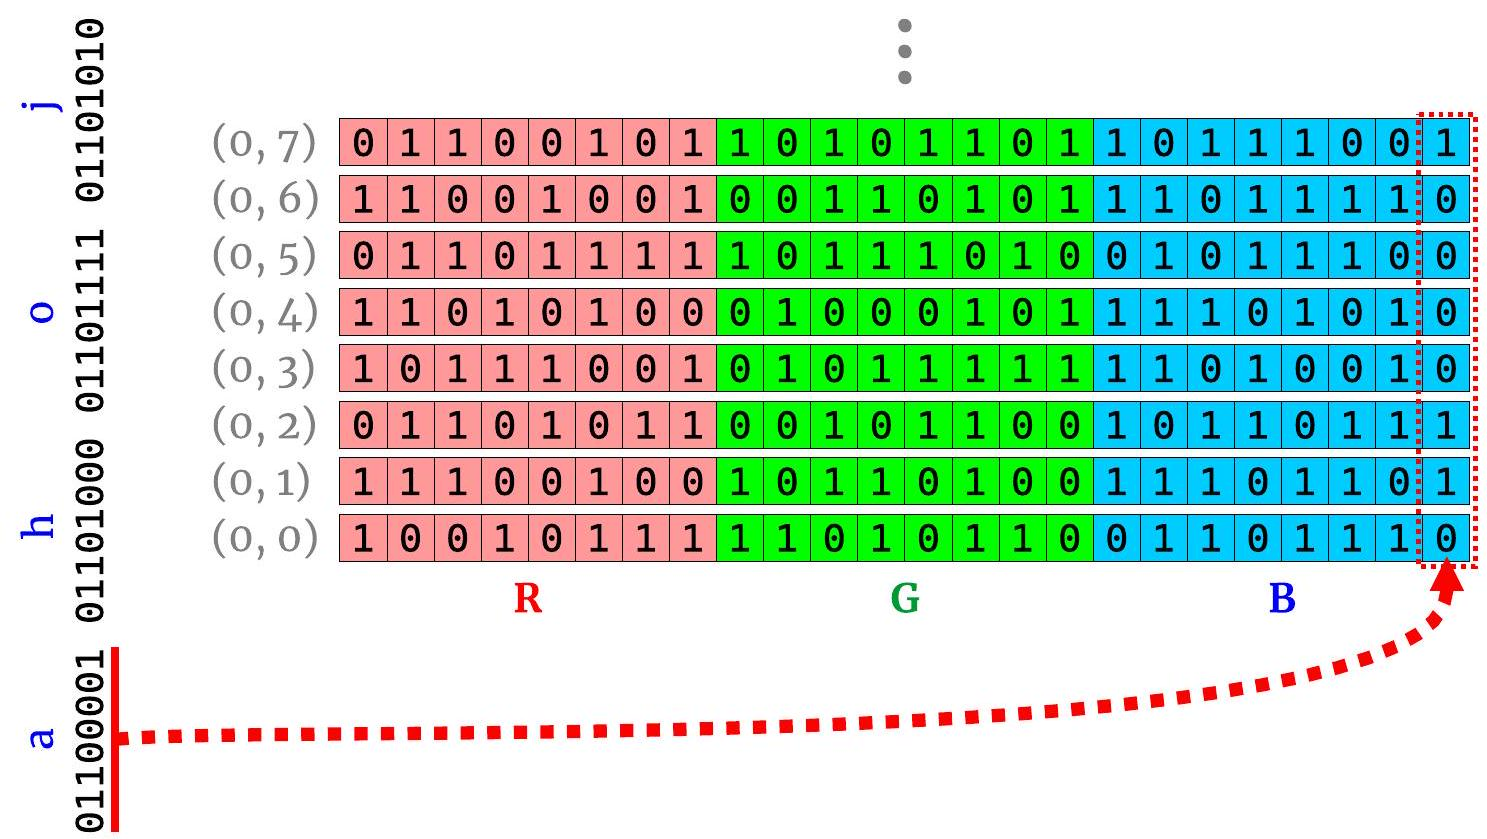
\includegraphics[width=.8\textwidth]{zadani_LSB.jpg}
        \caption{Ukázka způsobu steganografického kódování textu do RGB bitmapy:\url{https://www.kiv.zcu.cz/studies/predmety/pc/data/works/sw2023-02.pdf}}

    \end{figure}

    se tedy před skrýváním textu do obrázku nejprve přesvědčí, že je obrázek (PNG nebo BMP) v subformátu 24-bit RGB (není-li toto splněno, ukončí se s chybovým hlášením), pak provede kompresi payloadu bezeztrátovou kompresní technikou LZW, ověří, že se zkomprimovaný obsah „vejde" do pixelů obrázku (tj. zda je jich dostatek - pokud ne, opět se ukončí s chybovým hlášením) a nakonec zkomprimovaný obsah uloží naznačeným způsobem do bitmapy, kterou zapíše na disk.\\

Program se bude spouštět příkazem\\

    \texttt{\textbf{stegim.exe}} \footnote{Přípona .exe je povinná i při sestavení v Linuxu, zejm. při automatické kontrole validačním systémem.}$\langle$ \textit{obrázek} $[\cdot \mathrm{\texttt{\textbf{png}}} \mid$. \texttt{\textbf{bmp}}] $\rangle\langle-$ \textit{přepínač směru} $\rangle\langle$ \textit{payload} $\rangle$\\

    Symbol 〈\textit{obrázek}〉 zastupuje první povinný parametr - název souboru s bitmapovým obrázkem ve formátu PNG nebo BMP, subformátu 24-bit RGB, do kterého bude steganograficky ukryt nebo
    z něj bude naopak extrahován příslušný užitečný obsah (podle toho, jaký bude uveden přepínač směru).

    Symbol 〈-\textit{přepinač směru}〉 pak predstavuje druhý povinný parametr, kterým uživatel určuje, zda se bude payload ze souboru do obrázku zakódovávat nebo se bude z obrázku extrahovat a ukládat na disk. Je-li tento přepínač předán programu ve tvaru '\textbf{-h}' (jako\textit{ \textbf{h}ide}), bude payload specifikovaný třetím povinným parametrem komprimovat a ukrývat do obrázku. Při zadání ve tvaru '-\textbf{x}' (jako \textit{e\textbf{x}tract}) bude payload vyjímat z bitmapového obrázku, dekomprimovat a ukládat zpět na disk do zvoleného souboru (daného třetím povinným parametrem).

    Třetí povinný parametr zastoupený symbolem $\langle$ \textit{payload} $\rangle$ je specifikace souboru na disku, ze kterého program vezme užitečný obsah určený k ukrytí do obrázku nebo do něj naopak užitečný obsah vyjmutý z obrázku uloží.

    U obou předávaných souborů (obrázku a payloadu) berte v potaz možnost, že uživatel uvede jak krátké jméno, tak také úplnou specifikaci včetně úplné cesty (a ta může obsahovat i např. mezery).

    \href{https://www.kiv.zcu.cz/studies/predmety/pc/data/works/sw2023-02.pdf}{\textcolor{blue}{\underline{Podrobnější popis zde}}}

% ANALYZA ULOHY


    \chapter{Analýza úlohy}
    Při analýze úlohy vyvstává několik problémů, pro které je potřeba nalézt postup řešení. Nejdříve výběr kompresního alogritmu a poté zvolení vhodných datových struktur pro reprezentaci \textit{LZW slovníku} pro kompresy a dekompresy. Také zvolení datové struktury pro reprezentaci binárních dat. Poté způsob kontroly porušenosti dat.
    \section{Kompresní algoritmus}
    Pro kompresy dat mohlo být zvoleno mnoho algoritmů jako např. LZ77 nebo gzip, kde každý z nich má své výhody a nevýhody. Pro tento projekt byl zvolen kompresní algoritmus LZW z těchto důvodů:
    \begin{itemize}
        \item Využití tohoto algoritmu bylo definováno v zadání
        \item Předchozí znalost algoritmu a jeho předešlá implementace
        \item Vysoká Kompresní Účinnost: LZW dosahuje vysoké míry komprese dat, což je klíčovým kritériem v případě omezeného úložného prostoru nebo přenosové kapacity.
        \item Univerzálnost: LZW algoritmus je vhodný pro širokou škálu datových typů a formátů. To znamená, že může být použit v různých kontextech bez ohledu na specifické vlastnosti dat.
        \item Rychlá Implementace: Implementace LZW algoritmu je relativně jednoduchá a efektivní, což usnadňuje jeho rychlé začlenění do projektu.
    \end{itemize}

    \section{Datové struktury}
    Pro tento projekt bylo důležité zvolit vhodné datové struktury pro reprezentaci binárních dat a pro slovník LZW algoritmu.

    \subsection{Reprezentace binárních dat}
    Jelikož jazyk C nenabízí datový typ pro reprezentaci binárních dat je potřeba nalézt alternativu. 
    Binární data by se dala reprezentovat jako číslo co nabývá dvou hodnot(0, 1), ale to by zvýšilo nepřehlednost kódu a výsledné pole těchto znaků by bylo velice velké a následná konverze dat do jiných struktur by byla zbytečně náročná. 
    Proto pro tento projekt byla zvoleno dynamické pole s prvky uint8\footnote{číslo s velikostí 8 bitů}  se statickou inkrementací při nedostatku místa. Velikost jednoho prvku byla takto zvolena jelikož je to nejmenší možná datová struktura v jazyce C a reprezentuje jeden byte. Výhody tohoto řešení jsou, že se soubor jednoduše načítá do tohoto pole a při konverze na jiný typ dat lze jednoduše provést konverzi jen pomocí přetypování ukazatele.
    Pro pole těchto prvků mohl být zvolen \textit{linked list} nebo statické pole s dostatečnou velikostí nebo efektivnější dynamické pole (např. zvyšování o 2x násobek velikosti). Ale bylo zvoleno dynamické pole se zvyšováním velikosti o pevnou hodnotu, jelikož implementace této struktury je jednoduchá a díky tomu není náchylná na vytvoření chyb.
\subsection{Reprezentace slovníku LZW algoritmu pro kompresy}
Slovník LZW algoritmu pro kompresy je reprezentován jako \textit{trie} s 256 potomky \footnote{Jelikož LZW algoritmus reprezentuje data jako slova složená z písmen a ty se reprezentují jako 8 bitové číslo, takže existuje 256 možností} kde každý potomek reprezentuje znak, který následně jako hodnotu \textit{trie} obsahuje kód. Při slově delším než jeden znak se \textit{trie} následně rozšiřuje na další potomky.
Pro tuto strukturu je potřeba aby byl možný rychlí přístup ke kódu na základě slova a aby struktura neměla statickou velikost jelikož velikost slovníku se liší pro různá data.
Alternativy pro toto řešení jsou dynamické pole, linked list, hashovací tabulkou. Dynamické pole je nejjednoduší řešení, ale díky pomalému přístupu k jednotlivým prvkům je nevhodné. Linked list má také pomalý přístup k jednotlivým prvkům. Slovník by mohl být reprezentován hashovací tabulkou, kde by slovo bylo klíč a kód slovníku uložen jako hodnota jedné položky. Řešení hashovací tabulkou je také vhodné řešení pro toto použití, ale díky náročné implementaci byla zvolena trie.

\subsection{Reprezentace slovníku LZW algoritmu pro dekompresy}
    Pro názornost a jednoduchost v kódu je slovník LZW při dekompresy reprezentován jako pole  kde každý prvek obsahuje hodnotu reprezentovanou jako řetězec a jeho index je kód LZW slovníku.
    Toto pole je implementováno jako dynamické pole se pevnou inkrementací o konstantu. 
    Alternativy tohoto řešení by byla hash mapa, linked list nebo dynamické pole s jiným způsobem inkrementace. 
    Bylo zvoleno dynamické pole jelikož zajišťuje rychlý přístup k jednotlivým prvkům pomocí indexu, který je stejný jako kód LZW slovníku.


    \section{Kontrola porušenosti ukrytých dat}
    V rámci řešení bylo potřeba zvolit způsob jak zajistit že načtená data z obrázku nebyla poškozena manipulací s obrázkem.
\subsection{Parity byte}
Parita bytu, jako jednoduchá forma kontrolního součtu, nachází své využití v rámci detekce chyb v binárních datech. Paritní bit, buď sudý nebo lichý, je přidán k datům tak, aby vytvořil sudý nebo lichý počet jedniček v celkovém binárním vzoru. Tímto způsobem lze snadno detekovat chyby, zejména jednoduché bitové chyby, při přenosu nebo ukládání dat. Výhodou parity je její jednoduchá implementace a nízká náročnost na zpracování.

    Nicméně, existují i některé významné nevýhody spojené s použitím parity pro kontrolu integrity dat. Jednou z hlavních nevýhod je omezená schopnost opravovat chyby. Parita umožňuje pouze detekci chyb, ale neumožňuje identifikovat konkrétní chybové bity nebo je opravit. Navíc, parita je náchylná k detekci pouze lichého počtu jednotlivých bitových chyb; dvě a více chyb, které se vzájemně vyruší, mohou zůstat nezaznamenány.

    V dnešní době, s rostoucí složitostí a náročností na spolehlivost přenosu dat, moderní kontrolní součty nebo kódování s opravnou schopností mohou poskytovat lepší možnosti pro zajištění integrity dat v komunikačních nebo ukládacích systémech. Zatímco parita byla historicky důležitým nástrojem, moderní aplikace často volí robustnější a výkonnější metody pro kontrolu integrity dat.
    \cite{Checksum4:online}
\subsection{ Kontrolní součet}
Kontrolní součet, konkrétně doplněný součet (sum complement), slouží k zajištění integrity dat tím, že vytváří kontrolní hodnotu, která je odvozena z aritmetické operace nad daty. Jednou z hlavních výhod je relativně jednoduchá implementace a snadná výpočetní realizace, což umožňuje rychlé ověření integrity dat. V případě doplněného součtu jsou data sečtena, a následně je výsledek complementován. Získaný kontrolní součet je pak připojen k datům a může být použit pro kontrolu integrovanosti při přenosu nebo ukládání.

    Nicméně, metoda doplněného součtu má své omezení. Především je citlivá na početní přetečení (overflow), což může způsobit ztrátu informace o chybě. Tato metoda také neumožňuje identifikovat nebo opravit konkrétní chyby, ale pouze indikuje, že chyba nastala. Navíc, při použití pro binární data, může být náchylná k chybám v přenosu bitů, které se vzájemně vyruší a neprojeví se v kontrolním součtu.

    V moderních systémech, kde je kladen větší důraz na spolehlivost přenosu dat, se často upřednostňují sofistikovanější kontrolní součty nebo metody kódování s opravnou schopností, které jsou schopny detekovat a někdy i opravit chyby. I přes omezení je však doplněný součet stále používán v jednodušších aplikacích, kde je dostačující jednoduchost a nízká náročnost na zpracování.
   \cite{Checksum4:online}
\subsection{CRC}
    -- Kontrolní součet CRC (Cyclic Redundancy Check) představuje robustnější a sofistikovanější metodu pro kontrolu integrity dat. Na rozdíl od jednoduchých součtů, CRC je schopen identifikovat a detekovat různé typy chyb, včetně chyb ve formě jednotlivých bitů, změn v pořadí bitů nebo náhodných chyb. Je to dáno použitím polynomu, kterým se data násobí při výpočtu kontrolní hodnoty.

    Jednou z hlavních výhod CRC je jeho schopnost detekce chyb v rozsáhlejších datech a schopnost poskytnout vyšší úroveň spolehlivosti. Kromě toho CRC umožňuje identifikovat místo a povahu chyb, což usnadňuje diagnostiku problémů při přenosu nebo ukládání dat. Další výhodou je, že CRC je standardizovaný a používaný ve mnoha komunikačních protokolech a souborových formátech.

    Omezení metody CRC mohou zahrnovat vyšší nároky na výpočetní výkon v porovnání s jednoduchými součty. Nicméně, moderní výpočetní prostředky jsou obvykle dostatečně výkonné a umožňují efektivní výpočet CRC bez značného zvýšení nákladů. Vzhledem k jeho výkonu a rozšířenému použití se CRC stává preferovanou volbou pro kontrolu integrity dat v komplexnějších systémech.
    \cite{Cyclicre48:online}
\subsection{Secure Hash Algorithms}
Secure Hash Algorithms (SHA), zejména SHA-256 nebo SHA-3, představují silné nástroje pro kontrolu integrity dat v důsledku své odolnosti proti kryptoanalýze a vlastnostem odolným vůči kolizím. Tyto algoritmy vytvářejí unikátní hashové hodnoty pro vstupní data, což znamená, že i malá změna ve vstupech vytvoří zcela odlišnou hashovou hodnotu. Tímto způsobem lze s vysokou pravděpodobností detekovat jakoukoli změnu v datech.

    Hlavní výhodou SHA oproti jednoduchým kontrolním součtům je jeho schopnost odolávat pokročilým útokům, jako jsou kolizní útoky. Tyto algoritmy jsou navrženy tak, aby byly odolné vůči nelegitimním pokusům o vytvoření dvou různých vstupů se stejnou hashovou hodnotou. SHA algoritmy jsou standardizované a používají se v široké škále bezpečnostních aplikací a protokolů.

    Omezení použití SHA mohou zahrnovat nároky na výpočetní výkon, zejména u složitějších variant algoritmů. Nicméně, moderní hardwarová a softwarová řešení obvykle umožňují efektivní výpočty SHA. Další omezení může spočívat v tom, že hashové hodnoty jsou pevně dané délky, což někdy může být nepraktické pro určité aplikace.

    Celkově lze říci, že Secure Hash Algorithms poskytují vyšší úroveň bezpečnosti a spolehlivosti při kontrole integrity dat, což je zvláště důležité v citlivých bezpečnostních a kryptografických kontextech.
   \cite{SecureHa61:online}
\subsection{MD5}
MD5 bylo historicky využíváno pro vytváření unikátních hashových hodnot pro vstupní data. Jedná se o algoritmus, který rychle generuje 128bitové hashové hodnoty. Jednou z jeho původních výhod byla rychlost a jednoduchost implementace. MD5 bylo široce používáno k ověření integrity souborů nebo hesel.

    Nicméně, v posledních letech bylo objeveno několik zranitelností v návrhu MD5, což způsobilo, že se stalo náchylným k tzv. kolizním útokům. Kolizní útoky umožňují vytvoření dvou různých vstupních sad dat, které generují stejný hash. To zpochybnilo původní zamýšlené použití MD5 pro bezpečnostní účely, jako je ověřování integrity nebo digitální podpisy.

    Dnes se nedoporučuje používat MD5 pro bezpečnostní aplikace, kde je nutná odolnost proti kolizím a bezpečnost dat. I přes svou historickou relevanci v rychlém generování hashových hodnot má MD5 v současné době omezené uplatnění v bezpečnostních scénářích. Modernější algoritmy, jako SHA-256 nebo SHA-3, jsou nyní preferovanou volbou, a to zejména tam, kde je bezpečnost klíčovým faktorem.
    \cite{MD5Wikip50:online}

\subsection{Volba}
    Jelikož Parity byte a sum complement nejsou dostačující pro ověření jestli nebyla data výrazně poškozena pro tento projekt bylo zvolen crc přímo crc32 díky předešlé znalosti této checksumy a její implementace a taktéž jelikož díky knihovně \textit{zlib.h} je implementace do programu snadná. SHA a MD5 nebyli zvoleny kvůli náročnosti implementace do tohoto projektu i když jsou to vhodné alternativy.


% POPIS IMPLEMENTACE


    \chapter{Popis implementace}
 
\section{   Moduly}
    Hlavní spuštění probíhá v main.c
    
   
\subsection{Hlavní moduly}
    \begin{itemize}
        \item Main
        \item Compression
        \item Image
        \item Payload
    \end{itemize}

    Moduly si mezi sebou předávají pouze \textit{payloadarray} datový typ, který reprezentuje binární pole.
   
\subsection{Pomocné moduly}
    Ve složce utils jsou vytvořeny pomocné funkce pro tuto aplikaci.
    \begin{itemize}
        \item BinaryData
        \begin{itemize}
            \item Zde jsou implementovány datové struktury pro práci s binárními daty
        \end{itemize}
        \item Dictionary
        \begin{itemize}
            \item Zde jsou implementovány datové struktury pro kompresy pro modul Compression
        \end{itemize}
        \item Trie
        \begin{itemize}
            \item Zde je implementována datová struktura trie pro slovník lzw algoritmu pro kompresy
        \end{itemize}
        \item Logger
        \begin{itemize}
            \item Zde jsou implementovány funkce pro vypisování chyb a jiných zpráv do konzole
        \end{itemize}
        \item Memory Management
        \begin{itemize}
            \item Zde jsou implementovány wrapper funkce pro allokování a dealokování paměti v aplikaci
        \end{itemize}
        \item Utils
        \begin{itemize}
            \item Zde jsou implementovány ostatní pomocné funkce pro práci s řetězci a soubory
        \end{itemize}
        \begin{itemize}
            \item Tento modul vkládá do sebe moduly \textit{logger} a \textit{memory management} a následně se vkládá již jen tento modul do ostatních souborů
        \end{itemize}
    \end{itemize}


 
    
\section{Průběh programu a komunikace modulů}
    
\subsection{Ukrytí dat - interakce modulů}
    \begin{enumerate}
        \item \textit{Main} předá \textit{Payload} jméno souboru s payload daty a \textit{Payload} tato data připraví a vrátí jako binární pole \textit{payloadarray}  
        \begin{enumerate}
            \item modul \textit{Payload} při přípravě dat využije modul \textit{Compression} kterému předá binární pole \textit{payloadarray} a modul \textit{Compression} vrátí binární pole se zkomprimovanými daty
        \end{enumerate}
        \item připravené binární pole předá \textit{Main} do modulu \textit{Image} spolu se jménem souboru obrázku a \textit{Image} uloží tyto data do obrázku
    \end{enumerate}
    
\subsection{Extrakce dat - interakce modulů}
    \begin{enumerate}
        \item \textit{Main} předá jméno souboru obrázku se schovanými daty modulu \textit{Image} a ten vrátí binární pole \textit{payloadarray}  se schovanými daty extrahovanými z obrázku
        \item \textit{Main} toto pole předá modulu \textit{Payload} a ten vrátí původní data modulu \textit{Main} jako řetězec
        \begin{enumerate}
            \item  modul \textit{Payload} při přípravě dat zavolá modul \textit{Compression} kterému předá řetezec a modul \textit{Compression} mu předá dekomprimovaný řetězec
        \end{enumerate}
        \item \textit{Main} uloží tato data do výstupního souboru
    \end{enumerate}

    \section{Modul: Compression}
    Tento modul implementuje funkce pro kompresy a dekompresy binárních dat pomocí algoritmu LZW. 

    \subsection{LZW algoritmus}
    LZW algoritmus je unikátní kompresní technikou, která se zaměřuje na identifikaci opakujících se vzorů v datovém proudu a následně na jejich nahrazení krátkými kódy. Klíčovým principem algoritmu je vytváření slovníku, do kterého jsou postupně přidávány nové vzory. Pokud je nějaký vzor v datovém proudu identifikován, je nahrazen odpovídajícím kódem ze slovníku, což výrazně snižuje objem dat. LZW se tímto způsobem adaptuje na strukturu dat a může dosáhnout vysoké míry komprese.

    Jednou z klíčových výhod LZW algoritmu je jeho schopnost dosáhnout významné komprese dat bez ztráty informací. Tato metoda je široce používána v kompresních formátech, jako je například GIF pro obrázky nebo TIFF. Další výhodou je rychlá implementace, která umožňuje efektivní kompresi dat s minimálním zpožděním.

    Nicméně, je třeba poznamenat, že LZW je bezkontextový algoritmus, což znamená, že každý symbol je komprimován nezávisle na kontextu okolních symbolů. Toto může způsobit, že LZW nemusí být vždy nejúčinnější pro všechny typy dat. \cite{Lempel–Z75:online} \cite{LZWLempe46:online}

    \subsubsection{LZW komprese}
Implementace komprese je v tomoto projektu podle tohoto pseudokódu.
\begin{samepage}
    \begin{mdframed}
        \begin{minted}[linenos]{shell}
Initialize table with single character strings

     P_INPUT_CHAR = first input character
     
     WHILE not end of input stream
     
          C_NEXT_CHAR = next input character
         
          IF P_INPUT_CHAR + C_NEXT_CHAR is in the string table
          
            P_INPUT_CHAR = P_INPUT_CHAR + C_NEXT_CHAR
            
          ELSE
          
            output the code for INPUT_CHAR
            
            add P_INPUT_CHAR + C_NEXT_CHAR to the string table
          
            P_INPUT_CHAR = C_NEXT_CHAR
          
     END WHILE
     
    output code for P_INPUT_CHAR
        \end{minted}
    \end{mdframed}
    \end{samepage}
    

    \subsubsection{LZW dekomprese}
    Implementace dekomprese je v tomoto projektu podle tohoto pseudokódu.
    \begin{samepage}
    \begin{mdframed}
        \begin{minted}[linenos]{shell}
Initialize table with single character strings

OLD = first input code
save to result translation of OLD

WHILE not end of input stream
NEW = next input code
IF NEW is not in the string table
S = translation of OLD
S = S + C
ELSE
S = translation of NEW
output S
C = first character of S
OLD_value + C to the string table
OLD = NEW
END WHILE
        \end{minted}
    \end{mdframed}
    \end{samepage}


    \section{Modul: Image}
    Tento modul implementuje metody pro schování a extrakci binárních dat z modré hodnoty LSB obrázku ve formátu .png a .bmp.
    Vždy ukládá a načítá data od prvního pixelu po délku připravených dat

    \subsection{LSB - Nejméně významný bit}
    "Ve výpočetní technice je nejméně významný bit (LSb nebo LSB[1] = least significant bit), který má v celém dvojkovém čísle váhu jedna. Nemusí jít pouze o proměnnou, ale také o registr nebo sběrnici v procesoru nebo v periferii. Jeho hodnota současně určuje lichost nebo sudost čísla.

    LSB se také označuje jako bit, který je nejvíce vpravo (right-most bit), což odpovídá běžné konvenci zápisu čísel zleva doprava, od číslice s nejvyšší váhou po číslici s nejnižší váhou. To odpovídá také celočíselným operacím "bitový posuv doleva", který odpovídá násobení dvojkou a "bitový posuv doprava", který odpovídá celočíselnému dělení dvojkou." \cite{Nejméněv98:online}

    \begin{figure}[h]

        \centering
        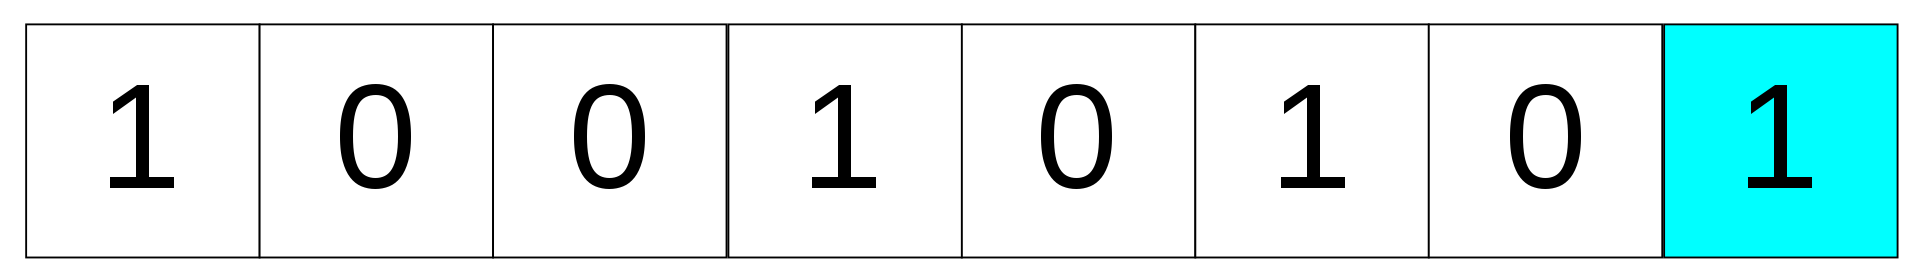
\includegraphics[width=.8\textwidth]{images/1920px-Least_significant_bit.svg (1).png}
        \caption{Zápis čísla 149 ve dvojkové soustavě se zvýrazněným nejméně významným bitem \url{https://upload.wikimedia.org/wikipedia/commons/thumb/a/a2/Least_significant_bit.svg/1920px-Least_significant_bit.svg.png}}

    \end{figure}

    V obrázcích tato hodnota vyjadřuje poslední bit modré číselné hodnoty v pixelu.

    \section{Modul: Payload}
    Tento modul zajišťuje za prvé zaobalení dat které mají být schovány se signaturou a kontrolní součet a následně využije modul \textit{Compression} pro kompresy schovaných dat. Tento modul vytváří kontrolní součet na základě zkomprimovaných dat pomocí CRC32.

    A za druhé získání ukrytých dat z dat která byla extrahována z obrázku a to odstraněním signatury a kontrolního součtu a následné dekomprese pomocí modulu \textit{Compression}. Tento modul současně kontroluje jestli je signatura validní a jestli je stejný kontrolní součet neboli jestli data nebyla poškozena.
\\
   \textbf{ Struktura dat ukládaných do obrázku}

    \begin{itemize}
        \item velikost dat v bytech - 4 byty
        \item signatura - 18 bytů
        \item kontrolní součet - 4 byty
        \item zkomprimovaná data pro ukrytí - podle hodnoty velikost dat v bytech
    \end{itemize}


    \section{Pomocný modul: BinaryData - datová struktura pro binární data}
    Tento modul implementuje strukturu \textit{binarydataarray} která reprezentuje binární data předávaná mezi moduly. Je realizována jako dynamické pole char kde každý element tohoto pole vyjadřuje 8 binárních znaků (jelikož char má velikost 1 byte). Je zde i funkce která vrací jednotlivé bity, které využívají bitové operátory pro získání specifického bytu z elementu. Také je zde funkce pro přidávání jednotlivých bytů do pole která postupně upravuje jednotlivé bity v elementech a přidává elementy podle potřeby pomocí bitových operátorů. Pole je realizováno jako dynamické a v okamžiku že je plné je inkrementováno o konstantu 1000 a realokována paměť.


    \section{Pomocný modul: Dictionary - datové strutury pro dekompresy}
    Tento modul implementuje datové struktury pro slovník LZW algoritmu při dekompresy.
    Je to realizováno jako struktura dynamického pole která za elementy obsahuje strukturu která představuje jeden slovníkový zápis a tento slovníkový element je tvořen z kódu (relizováno jako int 16 bitů) a hodnoty (realizováno jako řetězec). V okamžiku je je pole slovníkových zápisů plné zvýší se kapacita pole o konstantu a je realokována paměť.

    Pro reprezentaci polí slovníkových hodnot se taktéž používá dynamické pole s zvýšením kapacity o konstantu.
    Pro reprezentaci pole kódových hodnot se používá dynamické pole se statickou velikostí.
    Tyto struktury se využívají pro komunikaci mezi funkcemi v modulu \textit{Compression}

\section{Pomocný modul: Trie - datová struktura pro kompresy}
Zde je implementována datová struktura trie. 
Slovník LZW algoritmu pro kompresy je reprezentován jako \textit{trie} s 256 potomky \footnote{Jelikož LZW algoritmus reprezentuje data jako slova složená z písmen a ty se reprezentují jako 8 bitové číslo, takže existuje 256 možností} kde každý potomek reprezentuje znak, který následně jako hodnotu \textit{trie} obsahuje kód. Při slově delším než jeden znak se \textit{trie} následně rozšiřuje na další potomky.
% UZIVATELSKA PRIRUCKA


    \chapter{Uživatelská příručka}
    Tento program funguje na OS:
    Win32/64
    UNIX/Linux
    pro tyto systémy jsou připravené makefile

    Pro překlad tohoto projektu je potřeba mít nástroj pro překlad jazyka C (gcc, Microsoft Visual C/C++) a knihovnu libpng


    \section{Instalace překladače GCC}
    
\paragraph{Win32/64}
    \href{https://dev.to/gamegods3/how-to-install-gcc-in-windows-10-the-easier-way-422j}{https://dev.to/gamegods3/how-to-install-gcc-in-windows-10-the-easier-way-422j}
  
\paragraph{UNIX/Linux}
    \href{https://www.geeksforgeeks.org/how-to-install-gcc-compiler-on-linux/}{https://www.geeksforgeeks.org/how-to-install-gcc-compiler-on-linux/}


    \section{Instalace překladače Microsoft Visual C/C++}
    
\paragraph{Win32/64}

    \href{https://learn.microsoft.com/cs-cz/cpp/windows/latest-supported-vc-redist?view=msvc-170}{https://learn.microsoft.com/cs-cz/cpp/windows/latest-supported-vc-redist?view=msvc-170}
    
\paragraph{UNIX/Linux}
    \href{https://www.geeksforgeeks.org/how-to-install-visual-c-on-linux/}{https://www.geeksforgeeks.org/how-to-install-visual-c-on-linux/}


    \section{Instalace libpng}
    \href{http://www.libpng.org/pub/png/libpng.htm}{http://www.libpng.org/pub/png/libpng.html}


    \section{Postup Překladu}
    \begin{enumerate}
        \item Nainstalujte překladač GCC nebo Microsoft Visual C/C++ podle vašeho operačního systému
        \item Nainstalujte knihovnu libpng
        \item  Otevřete příkazový řádek na kořenovou složku projektu
        \item  Přeložte program pomocí příkazu make s jedním ze dvou souborů
        \begin{enumerate}
            \item \textit{ Makefile} pro GCC překladač
            \item \textit{  Makefile.win}) pro Microsoft Visual C/C++ s \textit{libpng.lib} v adresáři "C:/Program Files(x86)/GnuWin32/lib"
        \end{enumerate}
        \item  Spusťte program s vašimi parametry
    \end{enumerate}

    \section{Používání programu}
    V okamžiku že jste program přeložili můžete program spustit takto

    \texttt{\textbf{stegim.exe}} $\langle$ \textit{obrázek} $[\cdot \mathrm{\texttt{\textbf{png}}} \mid$. \texttt{\textbf{bmp}}] $\rangle\langle-$ \textit{přepínač směru} $\rangle\langle$ \textit{payload} $\rangle$\\

    Symbol 〈\textit{obrázek}〉 zastupuje první povinný parametr - název souboru s bitmapovým obrázkem ve formátu PNG nebo BMP, subformátu 24-bit RGB, do kterého bude steganograficky ukryt nebo
    z něj bude naopak extrahován příslušný užitečný obsah (podle toho, jaký bude uveden přepínač směru).

    Symbol 〈-\textit{přepinač směru}〉 pak predstavuje druhý povinný parametr, kterým uživatel určuje, zda se bude payload ze souboru do obrázku zakódovávat nebo se bude z obrázku extrahovat a ukládat na disk. Je-li tento přepínač předán programu ve tvaru '\textbf{-h}' (jako\textit{ \textbf{h}ide}), bude payload specifikovaný třetím povinným parametrem komprimovat a ukrývat do obrázku. Při zadání ve tvaru '-\textbf{x}' (jako \textit{e\textbf{x}tract}) bude payload vyjímat z bitmapového obrázku, dekomprimovat a ukládat zpět na disk do zvoleného souboru (daného třetím povinným parametrem).

    Třetí povinný parametr zastoupený symbolem $\langle$ \textit{payload} $\rangle$ je specifikace souboru na disku, ze kterého program vezme užitečný obsah určený k ukrytí do obrázku nebo do něj naopak užitečný obsah vyjmutý z obrázku uloží.

    \subsection{Příklady použití}

    \subsubsection{Operační systém Windows}

    \paragraph{Příklad 1: Ukrytí dat}
    \begin{itemize}
        \item \textbf{Zdrojový a cílový obrázek:} E:\textbackslash My Work\textbackslash Test\textbackslash Holiday 01.png
        \item \textbf{Přepínač směru:} -h
        \item \textbf{Soubor ukrývaný do obrázku:} secret\textbackslash text.txt
    \end{itemize}
     \texttt{\textbf{stegim.exe "E:\textbackslash My Work\textbackslash Test\textbackslash Holiday 01.png" -h secret\textbackslash text.txt}}

    \paragraph{Příklad 2: Extrakce dat}
    \begin{itemize}
        \item \textbf{Zdrojový a cílový obrázek:} E:\textbackslash Download\textbackslash Beach.bmp
        \item \textbf{Přepínač směru:} -x
        \item \textbf{Soubor ukrývaný do obrázku:} E:\textbackslash Documents\textbackslash Tajná zpráva.txt
    
    \end{itemize}
    \texttt{\textbf{stegim.exe "E:\textbackslash Download\textbackslash Beach.bmp" -x "E:\textbackslash Documents\textbackslash Tajná zpráva.txt"}}

    \subsubsection{Operační systém GNU/Linux, FreeBSD, macOS, atp}

    \paragraph{Příklad 3: Ukrytí dat}
    \begin{itemize}
        \item \textbf{Zdrojový a cílový obrázek:} /home/user/images/img001.png
        \item \textbf{Přepínač směru:} -h
        \item \textbf{Soubor ukrývaný do obrázku:} /home/user/doc/secret.txt
    \end{itemize}
\texttt{\textbf{stegim.exe /home/user/images/img001.png -h /home/user/doc/secret.txt}}

    \section{Ukončení programu}

    \subsection{Exit kód 0}
    Program úspěšně skončil.

    \paragraph{Výpis:}
    \begin{mdframed}
        \begin{minted}[linenos]{shell}
Hiding completed.
exit code 0
        \end{minted}
    \end{mdframed}

    \begin{mdframed}
        \begin{minted}[linenos]{shell}
Extraction completed.
exit code 0
        \end{minted}
    \end{mdframed}

    \subsection{Exit kód 1}
    Vyjadřuje nesprávně zadané či chybějící parametry na příkazové řádce (také
    neexistující vstupní/výstupní soubory)\\

    \paragraph{Výpis:}

    \begin{mdframed}
        \begin{minted}[linenos]{shell}
Wrong number of arguments - needed 3 arguments
You can use this program for hiding data in image or extract hidden data from image.
Hiding: stegim.exe <image_to_hide_to_filepath> -h <hide_payload_filepath>
Extraction: stegim.exe <input_image_to_extract_from_filepath> -x <output_payload_filepath>
exit code 1
        \end{minted}
    \end{mdframed}

    \begin{mdframed}
        \begin{minted}[linenos]{shell}
Invalid direction flag. Use -h for hiding or -x for extraction.
You can use this program for hiding data in image or extract hidden data from image.
Hiding: stegim.exe <image_to_hide_to_filepath> -h <hide_payload_filepath>
Extraction: stegim.exe <input_image_to_extract_from_filepath> -x <output_payload_filepath>
exit code 1
        \end{minted}
    \end{mdframed}

    \begin{mdframed}
        \begin{minted}[linenos]{shell}
Unable to hide the payload into the image.
Files doesnt exist or cannot be open.
exit code 1
        \end{minted}
    \end{mdframed}

    \begin{mdframed}
        \begin{minted}[linenos]{shell}
Unable to extract the payload from the image.
Files doesnt exist or cannot be open.
exit code 1
        \end{minted}
    \end{mdframed}

    \subsection{Exit kód 2}
    Vyjadřuje nevhodný formát obrázku (tj. není to PNG či BMP, 24-bit/pixel,
    RGB).\\

    \paragraph{Výpis:}

    \begin{mdframed}
        \begin{minted}[linenos]{shell}
Unable to hide the payload into the image.
Input file is not BMP or PNG 24 bit color.
exit code 2
        \end{minted}
    \end{mdframed}

    \begin{mdframed}
        \begin{minted}[linenos]{shell}
Unable to extract the payload from the image.
Input file is not BMP or PNG 24 bit color.
exit code 2
        \end{minted}
    \end{mdframed}

    \subsection{Exit kód 3}
    Vyjadřuje že obrázek není dostatečně velký pro ukrytí zadaného payloadu a
    potřebných doprovodných informací.

    \paragraph{Výpis:}

    \begin{mdframed}
        \begin{minted}[linenos]{shell}
Unable to hide the payload into the image.
Payload is too big for image.
exit code 3
        \end{minted}
    \end{mdframed}

    \subsection{Exit kód 4}
    Vyjadřuje že obrázek určený k extrakci payloadu neobsahuje žádný ukrytý ob-
    sah.\\

    \paragraph{Výpis:}

    \begin{mdframed}
        \begin{minted}[linenos]{shell}
Unable to extract the payload from the image.
Image doesnt have payload inside.
exit code 4
        \end{minted}
    \end{mdframed}

    \subsection{Exit kód 5}
    Vyjadřuje že ukrytý obsah byl poškozen, neodpovídá kontrolní součet obsahu
    či nelze obsah korektně dekomprimovat\\

    \paragraph{Výpis:}

    \begin{mdframed}
        \begin{minted}[linenos]{shell}
Unable to extract the payload from the image.
Hidden file in image was corrupted.
exit code 5
        \end{minted}
    \end{mdframed}

    \subsection{Exit kód 6}
    Vyjadřuje jakoukoli jinou chybu (alokace, špatné argumenty ve funkci)\\

    \paragraph{Výpis:}

    \begin{mdframed}
        \begin{minted}[linenos]{shell}
Unable to hide the payload into the image.
Other error.
exit code 6
        \end{minted}
    \end{mdframed}

        \begin{mdframed}
            \begin{minted}[linenos]{shell}
Unable to extract the payload from the image.
Other error.
exit code 6
            \end{minted}
        \end{mdframed}

% ZAVER


    \chapter{Závěr}
    Zadání projektu bylo splněno ve všech bodech. Program dokáže ukrýt data do obrázku typu BMP nebo PNG a následně i tyto data extrahovat z obrázku, který je obsahuje.

    Pro zlepšení rychlosti programu by pomohli vhodnější datové struktury jako např. HashMapa pro slovník LZW. Také by pomohlo efektivnější čtení souboru obrázku a načítání jeho dat.

    Problém při vývoji projektu nastal při čtení BMP souboru jelikož bylo špatně definované jeho čtení a rozdělení jeho částí. Problém byl i s nalezením všech úniků paměti a zajištění aby byla veškerá paměť uvolněna.


    \section{Časy běhu programu}

    \paragraph{Vstupní data}


    \begin{itemize}
        \item BMP obrázek: 29,5 kB
        \item PNG obrázek: 512 B
        \item Payload soubor: 32 B
    \end{itemize}

    \paragraph{Výsledky}
    \begin{itemize}
        \item Ukrytí do BMP souboru: 12.591 ms
        \item Ukrytí do PNG souboru: 11.156  ms
        \item Extrakce z BMP souboru: 4.872 ms
        \item Extrakce z PNG souboru: 5.570 ms
    \end{itemize}

    \bibliographystyle{plainurl}
    \bibliography{references}

% Seznamy obrázků a tabulek
    \listoffigures


\end{document}
